\section{Graphs and signals}

\subsection{Basic definitions}

\subsubsection{Graphs}

\begin{definition}\textbf{Graph}\\
A \emph{graph} $G$ is defined as a couple of sets $\langle V,E \rangle$ where $V$ is the set of \emph{vertices}, also called \emph{nodes}, and $E \subseteq\binom{V}{2}$ is the set of \emph{edges}. For all $u, v \in V$ we define the relation $u \sim v \Leftrightarrow \{u,v\} \in E$. Unless stated otherwise, we will consider only \emph{weighted} graphs \ie each graph $G$ is associated with a weight mapping $w: E \rightarrow \bbr^*$.
\end{definition}

\figref{fig:graph} illustrates an example of a graph. Note that we employ interchangeably the terms \emph{vertex} and \emph{node}.

\begin{figure}[H]
\centering
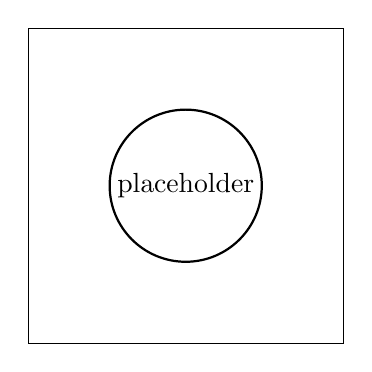
\begin{tikzpicture}
\draw (0,0) -- (4,0) -- (4,4) -- (0,4) -- (0,0);
\node at (2,2){placeholder};
\end{tikzpicture}
\caption{Example of a graph}
\label{fig:graph}
\end{figure}

\begin{remark}According to this definition, we consider simple graphs \ie no two edges share the same set of vertices and there is no self-loop.
\end{remark}

\begin{definition}\textbf{Path}\\
A \emph{path} of length $n \in \bbn$ in a graph $\gve$ is a sequence $(v_1 v_2 \cdots v_n)$ in $V$ such that $\forall i, v_i \sim v_{i+1}$.
\label{def:path}
\end{definition}

\begin{remark}Our definition of graphs admit no self-loop so $\forall i, v_i \neq v_{i+1}$
\end{remark}

\begin{definition}\textbf{Order}\\
The order of a graph $\gve$ is define as $\order(G) = |V| \in \bbn \cup \{+\infty\}$
\end{definition}

\begin{definition}\textbf{Adjacency matrix}\\
The \emph{adjacency matrix} of a finite graph $\gve$ of order $n$, is a $n \times n$ real-valued matrix $A$ associated to an indexing of $V = \{v_1, v_2, \ldots v_n\}$, such that
\begin{gather*}
A[i,j] =
 \begin{cases}
   w\left(\{v_i, v_j\}\right) & \text{if } v_i \sim v_j \\
   0 & \text{otherwise}
 \end{cases}
\end{gather*}
 \end{definition}

\begin{definition}\textbf{Degree}\\
The \emph{degree} of a vertex $v \in V$ of a graph $\gve$ is defined as $\deg(v) = |\{u \in V, u \sim v\}| \in \bbn \cup \{+\infty\}$.

The \emph{degree} of the graph $G$ is defined as $\deg(G) = \displaystyle \max_{v \in V}\{\deg(v)\}$.

A graph is said to be \emph{regular} if $\deg$ is constant on the vertices.
\end{definition}

\begin{definition}\textbf{Degree matrix}\\
The \emph{degree matrix} of a finite graph $\gve$ of order $n$, is the diagonal matrix $D$, associated to an indexing of $V = \{v_1, v_2, \ldots v_n\}$, such that $D = \diag(\deg(v_1), \deg(v_2), \ldots, \deg(v_n))$.
\end{definition}

\begin{definition}\textbf{Laplacian matrix}\\
The \emph{laplacian matrix} of a graph $\gve$ of order $n$, associated to an indexing of $V = \{v_1, v_2, \ldots v_n\}$, is defined as $L = D - A$, where $D$ is the degree matrix and $A$ is the adjacency matrix.
\end{definition}

\begin{definition}\textbf{Digraph}\\
A digraph is an oriented graph \ie $E \subseteq V \times V - \{(v,v), v \in V\}$. Contrary to a graph, the weight mapping $w$, the relation $\sim$, the adjacency matrix $A$, and the laplacian matrix $L$ are not symmetric. Notions defined on graphs naturally extends to digraphs where possible.
\end{definition}

\begin{definition}\textbf{Bipartite graph}\\
A \emph{bipartite graph} is a triplet of sets $\langle V^{(1)}, V^{(2)}, E \rangle$, where $V^{(1)}$ and $V^{(2)}$ are sets of vertices, $V^{(1)} \cap V^{(2)} \neq \emptyset$, and $E \subseteq V^{(1)} \times V^{(2)}$. It is associated with a weight mapping $w: E \rightarrow \bbr^*$. Its adjacency matrix $A$ is associated to indexings of $V^{(1)} = \{v^{(1)}_1, v^{(1)}_2, \ldots v^{(1)}_n\}$ and $V^{(2)} = \{v^{(2)}_1, v^{(2)}_2, \ldots v^{(2)}_n\}$, such that
\begin{gather*}
A[i,j] =
 \begin{cases}
   w\left((v^{(1)}_i,v^{(2)}_j)\right) & \text{if } (v^{(1)}_i,v^{(2)}_j) \in E \\
   0 & \text{otherwise}
 \end{cases}
\end{gather*}
\end{definition}

\begin{definition}\textbf{Induced subgraph}\\
The \emph{subgraph} $\widetilde{G} = \langle \widetilde{V},\widetilde{E} \rangle$ of a graph $\gve$, \emph{induced} by $\widetilde{V} \subseteq V$, is such that $\forall (u,v) \in \widetilde{V}^2, u \overset{\widetilde{G}}{\sim} v \Leftrightarrow u \overset{G}{\sim} v$.
\end{definition}

\begin{definition}\textbf{Grid graph}\\
A \emph{grid graph} $\gve$ is 
such that $V \cong \bbz^2$, $v_1 \sim v_2 \Rightarrow \|v_2 -v_1\|_\infty \in \{0, 1\}$ and either one of the following is true:
\begin{gather*}
\left\{
  \begin{array}{l}
    (i_1,j_1) \sim (i_2,j_2) \Leftrightarrow |i_2 - i_1| \XOR |j_2 - j_1| \quad \text{($4$ neighbours)}\\
    (i_1,j_1) \sim (i_2,j_2) \Leftrightarrow |i_2 - i_1| \AND |j_2 - j_1| \quad \text{($4$ neighbours)}\\
    (i_1,j_1) \sim (i_2,j_2) \Leftrightarrow |i_2 - i_1| \OR |j_2 - j_1| \quad \text{($8$ neighbours)}
  \end{array}
\right.
\end{gather*}

A \emph{(rectangular) grid graph} of size $n \times m$ is the subgraph of a grid graph induced by $\llbracket 1, n \rrbracket \times \llbracket 1, m \rrbracket$.

A \emph{square grid graph} is a rectangular grid graph of square size.
\end{definition}

\subsubsection{(Real-valued) Signals}

\begin{definition}\textbf{Signal space}\\
The \emph{signal space} $\cs(V)$, over the set $V$, is the linear space of real-valued functions defined on $V$.
\end{definition}

We have $\dim(\cs(V)) = |V| \in \bbn \cup \{+\infty\}$.

\begin{remark}
In particular, a vector space, and more generally a tensor space, are finite-dimensional signal spaces over any of their bases.
\end{remark}

\begin{definition}\textbf{Signal}\\
A \emph{signal} over $V$, $s \in \cs(V)$, is a function $s: V \rightarrow \bbr$.

An \emph{entry} of a signal $s$ is an image by $s$ of some $v \in V$ and we denote $s[v]$. If~$v$~is represented by a $n$-tuple, we can also write $s[v_1, v_2, \ldots, v_n]$.

The \emph{support} of a signal $s \in \cs(V)$ is $\supp(s) = \{ v \in V, s[v] \neq 0 \}$.
\end{definition}

\begin{definition}\textbf{Graph signal}\\ 
A \emph{graph signal} over $G$ is a signal over its vertex set. We denote by $\cs(G)$ the graph signal space.
\end{definition}

We have $\dim(\cs(G)) = \order(G) \in \bbn \cup \{+\infty\}$.

\begin{definition}\textbf{Underlying structure}\\
An \emph{(underlying) structure} of a signal $s$ over a set $V$, is a graph $G$ with vertex set $V$.
\end{definition}

\begin{remark}\textbf{Example of images, time series and graph signals}\\
When their is a unique clear underlying structure, we say it is \emph{the} underlying structure. For example, images are compactly supported signals over $\bbz^2$ and their underlying structure is a rectangular grid graph. Time series are signals over $\bbn$ and their underlying structure is a line graph. The underlying structure of a graph signal is obviously the graph itself.
\end{remark}

\subsection{Graphs in deep learning}

\todo{below}

We come across the notion of graphs several times in deep learning:
\begin{itemize}
\item Connections between two layers of a deep learning model can be represented as a bipartite graph, the \emph{connectivity graph}. It encodes how the information is propagated through a layer to another. See \secref{con_graph}.
\item Neural architectures can be represented by a graph. In particular, a computation graph is used by deep learning programming languages to keep track of the dependencies between layers of a deep learning model, in order to compute forward and back-propagation. See \secref{comp_graph}.
\item A graph can represent the underlying structure of an object (often a vector or a signal). The nodes represent its features, and the edges represent some structural property. See \secref{inductive_graph}.
\item Datasets can also be graph-structured. The nodes represent the objects of the dataset, and its edge represent some sort of relation between them. See \secref{transductive_graph}.
\end{itemize}

%\subsection{Graphs related to models}

\subsubsection{Connectivity graph}
\label{con_graph}

A Connectivity graph is the bipartite graph whose adjacency matrix is the connectivity matrix of a layer of neurons.
%$U = \{u_1, u_2, \ldots, u_n\}$
Formally, given a linear part of a layer, let $\textbf{x}$ and $\textbf{y}$ be the input and output signals, $n$ the size of the set of input neurons $N = \{u_1, u_2, \ldots, u_n\}$, and $m$ the size of the set of output neurons $M = \{v_1, v_2, \ldots, v_m\}$. This layer implements the equation $y = \Theta x$ where $\Theta$ is a $n \times m$ matrix.

\begin{definition}
{The \emph{connectivity graph} $G = (V,E)$ is defined such that $V = N \cup M$ and $E = \{(u_i,v_j) \in  N \times M, \Theta_{ij} \neq 0 \} $.}
\end{definition}

I.e. the connectivity graph is obtained by drawing an edge between neurons for which $\Theta_{ij} \neq 0$.
For instance, in the special case of a complete bipartite graph, we would obtain a dense layer. 
Connectivity graphs are especially useful to represent partially connected layers, for which most of the $\Theta_{ij}$ are $0$. 
For example, in the case of layers characterized by a small local receptive field, the connectivity graph would be sparse, and output neurons would be connected to a set of input neurons that corresponds to features that are close together in the input space. \figref{con_ex} depicts some examples.

\begin{figure}[h]
  \begin{center}
    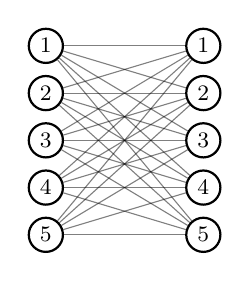
\begin{tikzpicture}
      \tikzstyle{every node} = [draw, circle, thick, inner sep = 2pt]
      \foreach \y in {0,...,4}{
        \pgfmathtruncatemacro{\yplusone}{5 - \y}
        \node(a\y) at (0,.6*\y) {\footnotesize\yplusone};
      }
      \foreach \y in {0,...,4}{
        \pgfmathtruncatemacro{\yplusone}{5 - \y}
        \node(\y) at (2,.6*\y) {\footnotesize\yplusone};
      }

      \foreach \x in {0,...,4}{
        \foreach \y in {0,...,4}{
          \path[opacity=0.5] (a\x) edge (\y);
        }
      }
    \end{tikzpicture}
  \end{center}
  \caption{Examples}
  \label{con_ex}
\end{figure}

\todo{\figref{con_ex}. It's just a placeholder right now}


Connectivity graphs also allow to graphically modelize how weights are tied in a neural layer. Let's suppose the $\Theta_ij$ are taking their values only into the finite set $K = \{w_1, w_2, \ldots, w_\kappa\}$ of size $\kappa$, which we will refer to as the \emph{kernel} of \emph{weights}. Then we can define a labelling of the edges $s: E \rightarrow K$. $s$ is called the \emph{weight sharing scheme} of the layer. This layer can then be formulated as $\displaystyle \forall v \in M, y_v = \sum_{u \in N, (u,v) \in E} w_{s(u,v)} x_u$. \figref{cnn} depicts the connectivity graph of a 1-d convolution layer and its weight sharing scheme.

\begin{figure}[h]
  \begin{center}
    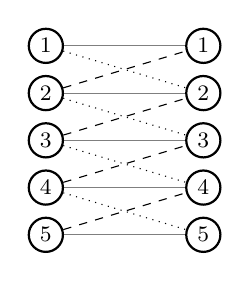
\begin{tikzpicture}
      \tikzstyle{every node} = [draw, circle, thick, inner sep = 2pt]
      \foreach \y in {0,...,4}{
        \pgfmathtruncatemacro{\yplusone}{5 - \y}
        \node(a\y) at (0,.6*\y) {\footnotesize\yplusone};
      }
      \foreach \y in {0,...,4}{
        \pgfmathtruncatemacro{\yplusone}{5 - \y}
        \node(\y) at (2,.6*\y) {\footnotesize\yplusone};
      }
      \path[opacity=0.5]
      (a0) edge (0);
      \path[dashed]
      (a0) edge (1);
      \path[dotted]
      (a1) edge (0);
      \path[opacity=0.5]
      (a1) edge (1);
      \path[dashed]
      (a1) edge (2);
      \path[dotted]
      (a2) edge (1);
      \path[opacity=0.5]
      (a2) edge (2);
      \path[dashed]
      (a2) edge (3);
      \path[dotted]
      (a3) edge (2);
      \path[opacity=0.5]
      (a3) edge (3);
      \path[dashed]
      (a3) edge (4);
      \path[dotted]
      (a4) edge (3);
      \path[opacity=0.5]
      (a4) edge (4);
    \end{tikzpicture}
  \end{center}
  \caption{Depiction of a 1D-convolutional layer and its weight sharing scheme.}
  \label{cnn}
\end{figure}


\todo{Add weight sharing scheme in \figref{cnn}}

\subsubsection{Computation graph}
\label{comp_graph}

%\subsection{Graphs related to data}

\subsubsection{Underlying graph structure and signals}
\label{inductive_graph}

\subsubsection{Graph-structured dataset}
\label{transductive_graph}

%transductive vs inductive